\documentclass{bioinfo}
\copyrightyear{2014}
\pubyear{2014}
\usepackage{xr}
\externaldocument{chipPCR}


\begin{document}
\firstpage{1}

\title[chipPCR]{chipPCR: an R Package to Pre-Process Amplification Curve Data}
\author[R\"odiger \textit{et~al.}]{Stefan R\"odiger\,$^{1}$\footnote{to whom correspondence should be addressed}, Micha\l{} Burdukiewicz\,$^{2}$ and Peter Schierack\,$^1$}
\address{$^{1}$Faculty of Natural Sciences, Brandenburg University of Technology 
Cottbus--Senftenberg, Senftenberg, Germany\\
$^{2}$Department of Genomics, Faculty of Biotechnology, University of 
Wroc\l{}aw, Wroc\l{}aw, Poland}

\history{Received on XXXXX; revised on XXXXX; accepted on XXXXX}

\editor{Associate Editor: XXXXXXX}

\maketitle

\begin{abstract}

\section{Motivation:}
The quantitative real-time polymerase chain reaction (qPCR) and quantitative 
isothermal amplification (qIA) are standard methods for quantification of 
nucleic acids. Numerous real-time read-out technologies with different technical 
foundation have been developed. Despite the continuous interest in amplification 
based techniques, there are only few tools for amplification data 
pre-processing. Especially, during development of new instruments a transparent 
tool for precise control of raw data is indispensable.

\section{Results:}
$\emph{chipPCR}$ is an \textbf{R} package for pre-processing and quality 
analysis of amplification curve data. The package takes advantage of 
\textbf{R}'s \emph{S4} object model and offers an extensible environment. 
It contains tools for the raw data exploration: functions to normalize, baseline, 
impute missing values, smooth amplification curves and a detect the start and end 
of an amplification curve. Capabilities of software are enhanced by implementation
of algorithms yet not present in \textbf{R}, as a 5-point stencil
for derivative interpolation. Simulation  tools, statistical tests, plots for data quality management, amplification efficiency/quantification cycle 
calculation, and 22 data sets from various qPCR and qIA experiments are also part of 
the package. The core functionalities of $\emph{chipPCR}$ are integrated in
GUI's (web-based and standalone \emph{shiny} applications) and for report 
generation.

\section{Availability:}
Stabel: http://cran.r-project.org/web/packages/chipPCR
Source code: https://github.com/michbur/chipPCR

\section{Contact:} \href{stefan.roediger@hs-lausitz.de}{stefan.roediger@hs-lausitz.de}

\section{Supplementary:} Supplementary data are available at Bioinformatics online.
\end{abstract}


\section{Introduction}

Quantitative polymerase chain reaction (qPCR) and quantitative isothermal 
amplification (qIA) are standard methods to amplify nucleic acids. These methods 
are used in real-time monitoring technologies, such as our previously reported 
VideoScan technology, microfluidic systems, point-of-care devices, and qPCR 
cyclers. Real-time technologies enable the quantification of nucleic acids by 
calculation of specific curve parameters like the quantification point (Cq) and 
the amplification efficiency (AE) 
\citep{roediger_highly_2013,rodiger_nucleic_2014,pabinger_2014}. Fundamental 
steps of amplification curve analysis are: (1) raw data read-in, (2) 
pre-processing (e.g., noise reduction), (3) amplification curve processing 
(e.g., Cq calculation), (4) post-processing and quantification, (5) data 
export/report generation. \textbf{R} belongs to the most used bioinformatic	
s tools and is a rapid adopter for various technologies like digital PCR, 
NanoString nCounter Platform, and qPCR \citep{waggott_2012,pabinger_2014}. Most 
qPCR \textbf{R} packages focus on the read-in and (post)-processing of data from 
commercial qPCR systems. \textbf{R} packages for the steps 1. and 3.--5. are 
available \citep{pabinger_2014,perkins_2012,mccall_2014,gehlenborg_2013}.

However, there is no \textbf{R} package for pre-processing and quality analysis 
of amplification curve data. Pre-processing is in most commercial cyclers a 
``black box'', which sets severe limits to reproducible research 
\citep{Leeper_2014}. Developmental qPCR and qIA technologies depend on tools to 
pre-process the raw data. Pre-processing algorithms remove stochastic errors and 
artefacts (Fig.~\ref{figure:problems}). Pre-processing addresses raw data 
inspection, raw data transformation in a format for successive analysis steps 
(e.g., smoothing, imputation), data reduction (e.g., removal of invalid sets) 
and data quality management. Misinterpretations are more likely if ``arbitrary'' 
corrections are performed. A manual alteration is in contradiction to 
reproducible research. The $\emph{chipPCR}$ package (``Lab-on-a-\textbf{Chip}'' 
\& \textbf{PCR}) was developed to fill this gab and to automatize 
pre-processing, data analysis/visualization and to offer a quality control for 
the statistical data analysis of qPCR and qIA experiments. \textbf{R} is very 
powerful to reproduce analysis on different platforms, to adopt to changing 
experimental setups and offers sophisticated statistical tools. Moreover, it is 
desirable to set up workflows in an open environment, which enables downstream 
analyses and which offers powerful tools for data visualizations and automatic 
report generation. The target audience encompasses developers and users who 
process raw data of commercial systems.

\section{Implementation}
\begin{methods}

$\emph{chipPCR}$ package was implemented in the \textbf{R} software environment 
as described elsewhere \citep{RCT_2013,rodiger_rkward_2012}. $\emph{chipPCR}$ is 
a relative of the \emph{MBmca} \citep{roediger_RJ_2013}, the $\emph{RDML}$  
\citep{blagodatskikh_2014}, and the \emph{dpcR} \citep{pabinger_2014} packages 
but focusses on pre-processing of amplification curves. The package contains 
pre-processor functions (smoothing, imputation, background correction, 
normalization), a function for single-blinded randomized rating, quality 
analysis summary functions, a function to calculate the amplification 
efficiency, and functions for amplification curve simulation, and report 
generation (Suppl. Sect.~\ref{sec:functions}). The supplemental material 
(packages vignette), uses Donald Knuth's literate programming 
principle~\citep{Knuth1984} to present the source code in a convenient way. 
$\emph{chipPCR}$'s naming convention is \textit{period.separated} 
\citep{Baaaath_2012}. We use \textbf{R}'s object model \emph{S4} class system 
(see \emph{methods} package) to separate between interface and implementation. 
It requires a higher effort than \emph{S3} classes, but assures better control 
on the object structure and the method dispatch. As a perquisite for 
high-throughput technologies, we avoided loops in the core structures and left 
options for partially parallel computing usage (\textsl{smoother} function) to 
keep the code fast. $\emph{chipPCR}$ includes a set of classes for plotting. The 
output of our custom made plots is minimalistic, but many parameters can be 
adjusted directly or by the ellipse parameter.

Our goal is to make our software available also for researchers not fluent in 
\textbf{R}. We implemented core functionality of our package in various 
GUI-technologies available in \textbf{R} \citep{rodiger_rkward_2012, 
shiny_2014}. Some of them are available as the web-based services. It is 
possible to run the GUI-applications as service on a server without installing 
\textbf{R} (e.g., http://michbur.shinyapps.io/MFIaggr\_gui/), on the local 
desktop (e.g., Fig.~\ref{figure:browser}), or as deployed from an external 
source for a local \textbf{R} installation. The functions \textsl{AmpSim}, 
\textsl{th.cyc}, \textsl{bg.max} and \textsl{amptester} are part of online GUIs. 
We hope to build monolithic systems to parse, pre-process and analyze 
amplification curve data in a combined work-flow. 

We have chosen not to rely on specialized parser but use native \textbf{R} 
workspaces, and dedicated \textbf{R} packages as default data format for import 
and export as described elsewhere \shortcites{perkins_2012, RCT_2013}. 
$\emph{chipPCR}$ presents \emph{S4} objects with tailored summary and plot 
methods. Data sets are an essential element of reproducible research 
\citep{Leeper_2014}. Our package contains 22 data sets from commercial and 
experimental cyclers along with the experimental settings (e.g., helicase 
dependent amplification (HDA)) (Suppl. Sect.~\ref{sec:XX}).
\end{methods}

\section{Example: quality analysis}

\textsl{MFIaggr} is a powerful analytical and graphical tool for fast multiple 
comparison of the cycle dependent signal dispersion and distribution 
(Fig.~\ref{fig:01}). The continuous response variable $y'_i$ is used to 
describe the relationships to one or more continuous predictor variables $y_1, 
..., y_n$. Use cases include the comparison of independent reaction vessels or 
the analysis of replicate experiments (Suppl. Sect.~\ref{sec:MFIaggr}). In 
particular, this function might be useful for quality management during the 
development of high-throughput technologies. An analysis via a the \emph{shiny} 
\textsl{MFIaggr.gui} app is shown in Fig.~\ref{figure:MFIaggr2}.

\begin{figure}[!tpb]%figure1
\centerline{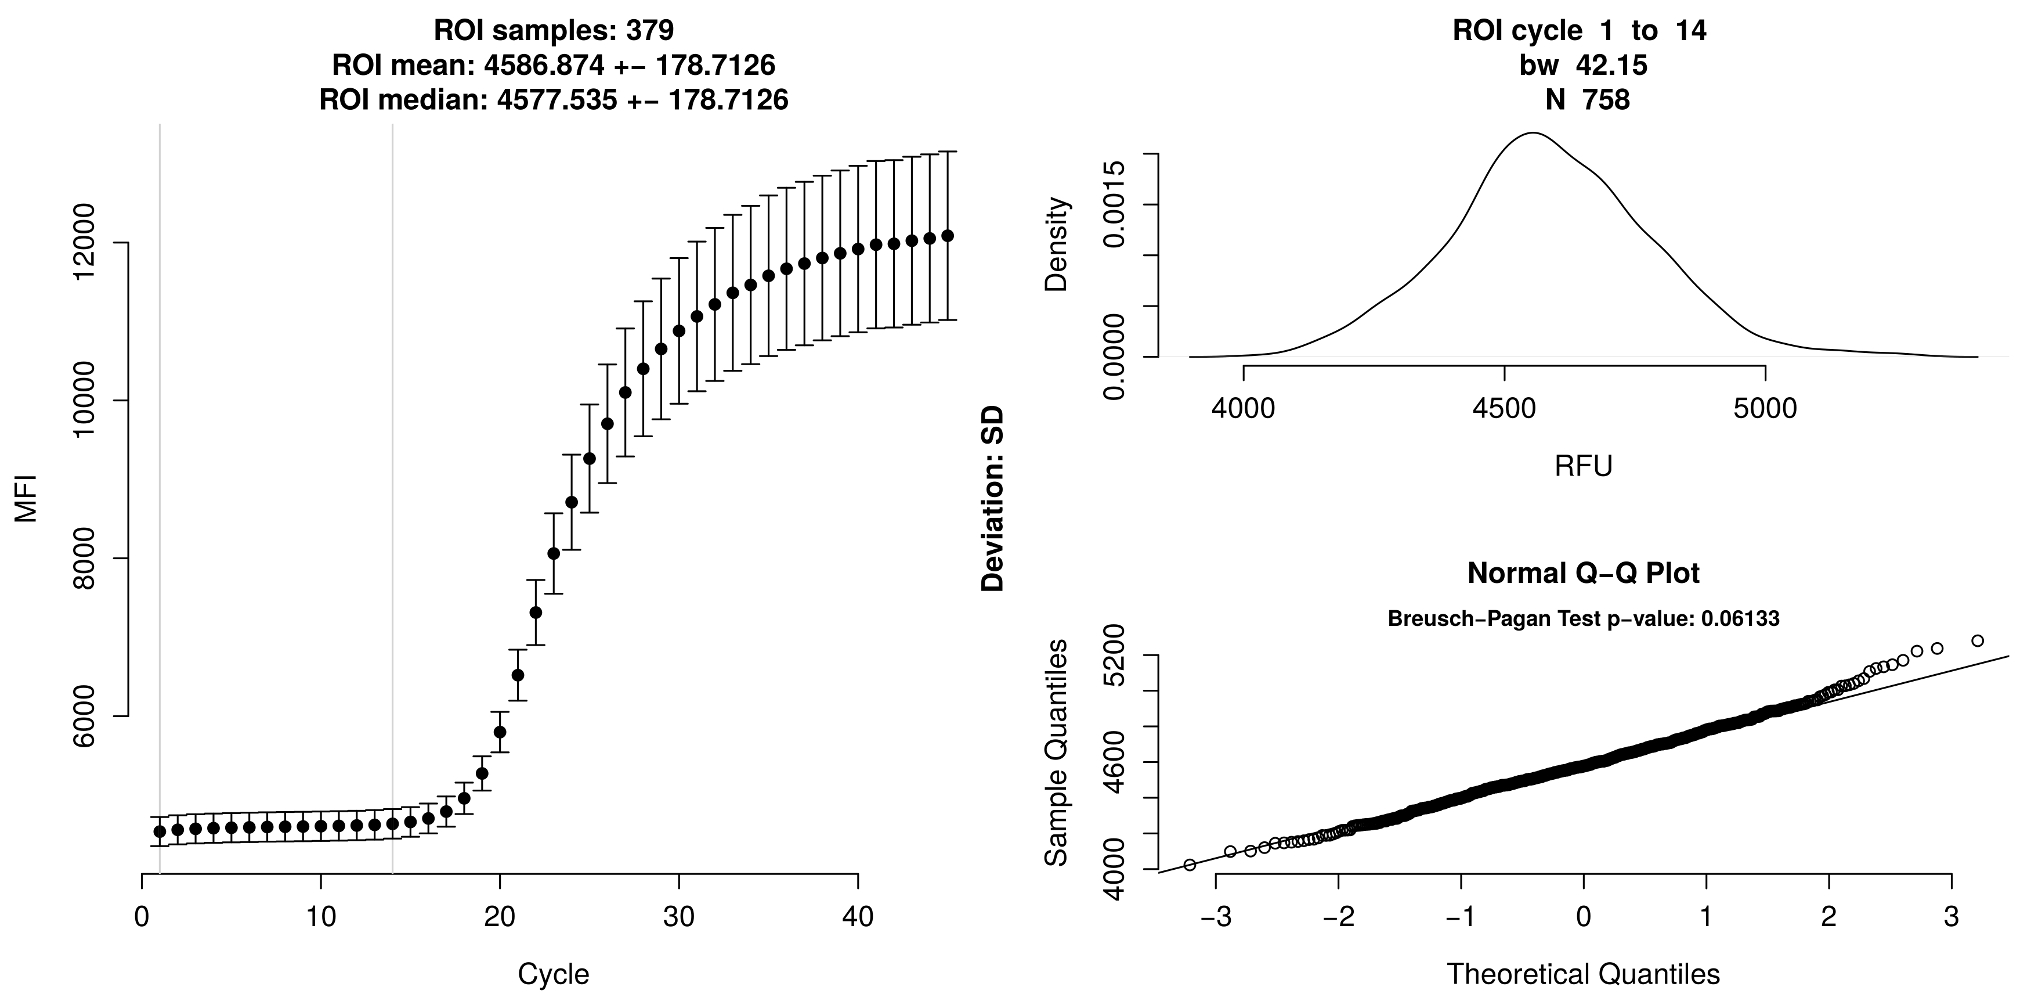
\includegraphics{fig01.jpg}}
\caption{Amplification curve analysis of 379 replicates. Cycles 1 to 14 was 
selected as region of interest (ROI) for \textsl{MFIaggr} to analyzes the 
cycle-dependent variance (left panel) and gives a density plot (right upper 
panel) and quantile-quantile analysis (right lower panel). The plots indicates 
that the data of the background range are normal distributed.}\label{fig:01}
\end{figure}

\section{Results and Conclusions}

There is an ongoing development for qPCR and qIA technologies. $\emph{chipPCR}$ 
is the first \textbf{R} package for the pre-processing and raw data quality 
analysis of amplification curve data of such systems. Though, $\emph{chipPCR}$ 
primarily targets pre-processing we also implemented standard methods to process 
amplification curve data. Functions of $\emph{chipPCR}$ are embeddable in 
customized routines with other packages (see Suppl.). For example, the packages 
\emph{dpcR} and \emph{MBmca} depend on $\emph{chipPCR}$ technology. 
$\emph{chipPCR}$ is build from smaller blocks. We claim that the modular 
structure of $\emph{chipPCR}$ package allows user to perform flexible data 
analysis adjusted to their needs. Users can do estimations by hand. For example 
for quantification cycle (second derivative maximum, $SDM$) estimation, solely 
the $\emph{chipPCR}$ functions \textsl{inder} and \textsl{smoother} are needed. 
\textsl{smoother} will be a method of smoothing in \textsl{inder} and by putting 
data in the \textsl{bg} object with summary method \textsl{summary-der} the user 
obtains the $SDM$. Thanks to the GUI it should be easy even for an users without 
any \textbf{R} experience omitting the biggest limitation of all \textbf{R} 
packages related to qPCR and qIA.


\section*{Acknowledgement}
Grateful thanks belong to the \textbf{R} community.

\paragraph{Funding\textcolon} This work was funded by the BMBF InnoProfile--Projekt 03 IPT 611X.

\paragraph{Conflict of Interest\textcolon} none declared.


\bibliographystyle{natbib}
%\bibliographystyle{achemnat}
%\bibliographystyle{plainnat}
%\bibliographystyle{abbrv}
%\bibliographystyle{bioinformatics}
%
%\bibliographystyle{plain}
%
\bibliography{Roediger_OxBio}
\end{document}
